\documentclass{report}

\usepackage[utf8]{inputenc} % un package
\usepackage[T1]{fontenc}      % un second package
\usepackage[francais]{babel}  % un troisième package
\usepackage{graphicx}       %un quatrième package
\graphicspath{ {C:/Users/alexandre/Documents/Cours/ESIEE/E3T/S1/P2/IGI-3006/} }

\title{Rapport de projet - IGE-3006}
\author{Alexandre \bsc{Causse} - Jérémy \bsc{Fornarino}}
\date{Année scolaire : 2016-2017}

\begin{document}

\maketitle

\renewcommand{\contentsname}{Sommaire} 
\tableofcontents
\listoffigures
\newpage

\chapter*{Introduction}
Le gomoku est un jeu de plateau consistant à aligner n pions sur les intersection d'un plateau de jeu de taille n*n.
Le but de ce projet est de créer un plateau de jeu pour le Gomoku et une intelligence artificielle capable d'évaluer l'efficacité de chaque coup afin de maximiser les chances de victoire.


\part{Rapport technique}
	\chapter{Présentation de choix technologiques}
		\section{Technologie utilisée}
		% Utilisation de Java, et de JavaFX pour l'ihm
Nous avons choisi comme langage de programmation Java car celui-ci nous semblait le plus adapté pour créer les différentes parties constituant le jeu.De plus ce langage nous permet, pour l'implémentation de l'interface homme machine, de nous servir de JavaFX et ainsi d'obtenir des rendus de bonne qualité et donc une meilleure expérience de jeu pour l'utilisateur.
		\section{Organisation du code}
		% --> Là on calle le diagramme de classe final en intro	
		%insérer diagramme de classes
		Dans cette partie nous allons exposer les différentes classes mises en jeu dans notre projet afin de comprendre l'architecture globale. 
\begin{figure}	\caption{\label{étiquette} diagramme de classes}
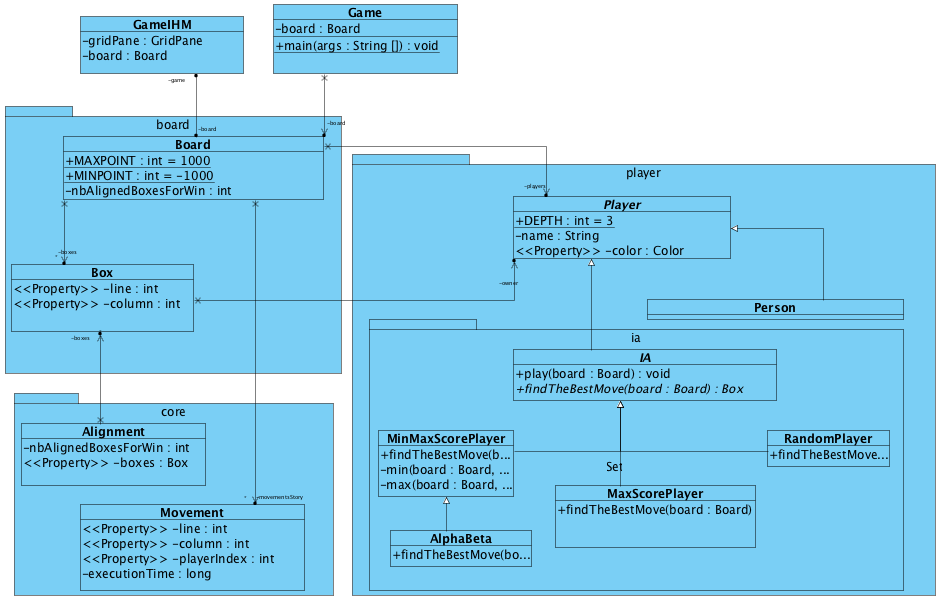
\includegraphics[scale=0.25]{diagrammeDeClasses.png} 
\end{figure}

			
			\subsection{Les classes principales}
			% --> Là on explique la classe Board, on passe très rapidement sur Game
			
			% --> Explication de la classe box
			% --> Explication de la classe Player et de la classe IA
			% % --> Pour les players il faut dire qu'elle definit une methode play, ce qui nous permet de ne pas avoir à la gerer ensuite d'un joueur à l'uatre, c'est rien d'autre que la structure et les methodes de bases
			% % --> La classe IA definit une structure predefinit pour l'ensemble des IA qu'on voudra mettre en place avec l'ajout de la methode "findTheBestMove", ce qui nous permet d'avoir différents algo possible dans notre programme et donc de pouvoir tester d'un algo à un autre
	    \subsection{Autres classes}
	        %---> alignment et movement
	\chapter{Description des algorithmes}
	%% ATTENTION : Bien parler de la pronfondeur, et expliquer que plus on va taper dans le fond plus l'algo est precis et a de chance de gagner, et moins il est rapide.
	Dans cette partie nous allons vous expliquer les différents algorithmes que nous avons décidé d'implémenter et d'utiliser dans notre projet.
		\section{Random}
		% --> Là on explique que pour commencer on a créer une IA Random, ca nous a permit de mettre en place la structure de notre code et de tester les différentes methodes relatives a la board en mettant de côté la phase algorithmiques qui viendra plus tard
		Cet algorithme va jouer de façon autonome sur n'importe quelle case libre du jeu de façon aléatoire. Il n'est pas très efficace car il ne prend pas en compte les coups joués par l'adversaire et ses chances de victoires sont assez faibles. Ainsi nous avons pensé à une première une première évolution qu'est le max score.
		\section{Max score}
		% Dans cette section nous expliquerons que on a commencé par créer un algorithme "max", cette alogrithmes permet de connaitre le coup qui nous rapportera le plus de point. On va expliquer comment il fonctionne (#schéma)
		% On concluera sur le fait que même si on a plus de chance de gagner grâce à cet algo, il pose des problèmes du fait qu'il ne prévoit pas que l'adversaire puisse gagner donc il ne lui bloquera pas ses coups
		% --> Transition en douceur vers l'algorithme MinMax
		Cet algorithme est la première étape permettant d'augmenter les chances de victoires. Le principe est qu'il cherche le meilleur coup (le "Max") à jouer pour gagner, celui qui rapportera le plus de points. Ainsi avec cette méthode les chances de victoires sont accrues cependant on peut lui reprocher de ne toujours pas prendre en compte les placements de pions de l'autre joueur et c'est cette dernière amélioration qui sera apportée dans l'algorithme suivant. 
		\section{Min Max}
		% Description de l'algorithme, explication de son fonctionement, l'avantage avec celui là
		% On concluera sur le fait que beaucoup de coup déjà connus son tout de même testés, et on fera une ouverture sur l'algorithme Alpha Beta, mais aussi sur celui qui permettrai de s'aretter en cas de match null avant la fin pour montrer qu'on a bien compris, et permettre des objets de recherches appronfu derriere #Impatable
        %ouverture temps execution
        Cet algorithme est le dernier fonctionnel que nous ayons implémenté. Il prend en paramètre un plateau de jeu et une profondeur d'arbre de jeu (cf schéma). Le principe est qu'il calcule à chaque tour le score maximum et le score minimum (correspondant respectivement au joueur courant et à l'adversaire). Cela signifie que cet algorithme suppose qu'à chaque tour, le joueur va effectuer le meilleur coup possible. La profondeur donnée au départ permet de spécifier jusqu'à quelle branche de l'arbre de jeu l'algorithme doit aller regarder. Ainsi plus on augmente la profondeur plus les chances de victoire sont grandes cependant cela à un coût de calcul impactant directement le temps d'exécution d'où l'idée de l'algorithme alpha-bêta.(cf partie à voir)
	\chapter{Les outils de test}
	% --> A voir si on a le temps de créer des tests en JUnit
	% --> A voir si on a le temps de faire tourner l'algo à mort pour montrer les tests statistiques

\part{Manuel d'utilisation}
	\chapter{Le développeur}
	% --> Là on peut revenir sur le fait que notre code est bien divisé et que si une personne veut reprendre notre architecture et simplement créer une IA sans se préocuper de la création de l'ensemble du jeux, c'est très simple, il suffit de créer une classe qui extends de IA. 
	% --> Pour lancer des parties qui se jouent seules il suffit de modifier dans Game.... Attention 
	La structure de ce projet à été pensé de telle sorte à permettre à un développeur d'implémenter une nouvelle intelligence artificielle de jeu sans avoir à se préocuper de la partie de gestion des tours, des joueurs. Pour cela il lui suffit de créer une nouvelle classe fille de la classe IA. Il pourra bénéficier de toutes les fonctionnalités de test déjà mises en place.
	
	

	\chapter{Le joueur}
	% --> Il suffit de lancer le jeux et bim bam boum, il lui suffit de jouer
	% --> A voir si on a le temps de revoir l'interface graphique pour permettre au joueur de choisir son nom, sa couleur, ainsi que l'IA qu'il affrontera

\part{Rapport d'activité}
% Utilisation de git
% On a beaucoup parlé, utilisation de schéma pour comprendre les algo
% Parler d'une première version avec des clones, et expliquer que le temps etait beaucou beaucoup beaucoup trop long pour être convenable 


\chapter*{Conclusion}





\end{document}